\resizebox{\textwidth}{!}{
	\begin{tikzpicture}[
		scale=.3,
		font={\footnotesize},
		node distance=.5,
		label distance=3pt,
		wide/.style={yscale=.75},
		net/.style={draw,trapezium,trapezium angle=75,inner sep=3pt},
		enc/.style={net,shape border rotate=270},
		dec/.style={net,shape border rotate=90},
		txt/.style={inner sep=3pt},
		loose/.style={looseness=.6},
		sg/.style={blue!60},
	]
	\matrix[
		tight,row sep=6,column sep=16,
		cells={scale=.3,},
	] {
		\&\&\&\&\&
		\node[dec] (guided-back) {guided \\ backprop}; \&
		\node[wide,label=90:$\ipder{_G L_C}{x}$] (guided) {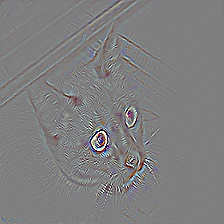
\includegraphics[width=.25\textwidth]{fig/gradient/fig/method/guided_gradient.jpg}}; \\
		\node[label=90:input image $x$] (in) {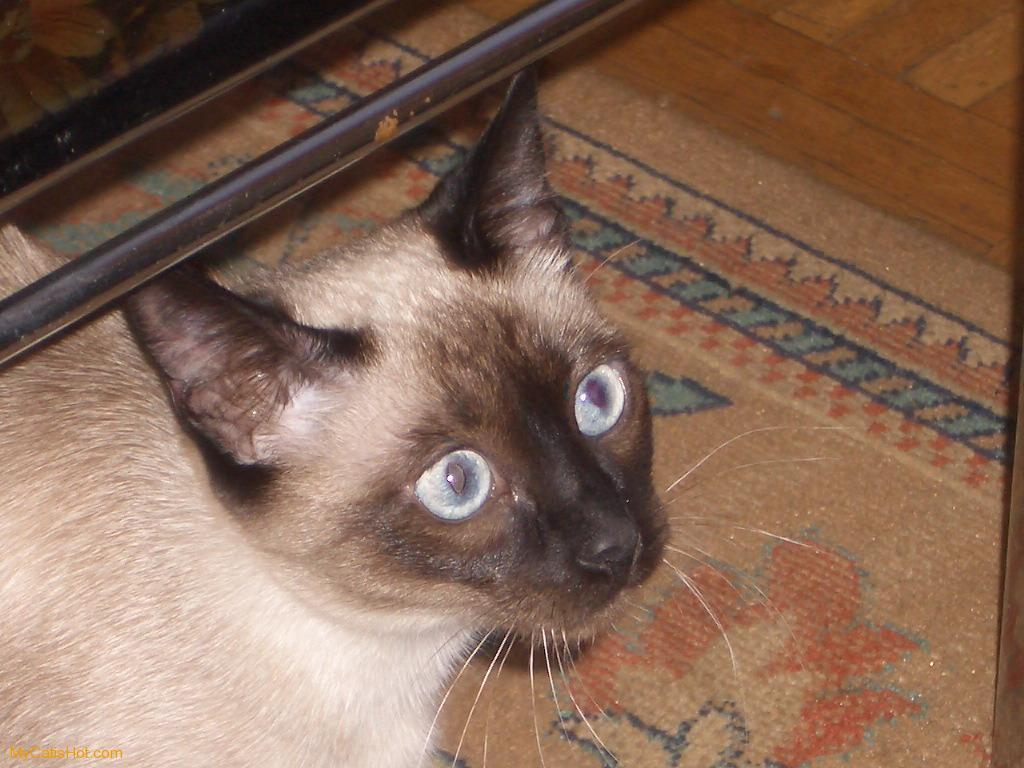
\includegraphics[width=.25\textwidth]{fig/gradient/fig/method/input.jpg}}; \&
		\node[enc] (net) {network \\ $f$}; \&\&\&
		\node[box] (class) {classification \\ loss $L_C$}; \&
		\node[dec] (back) {standard \\ backprop}; \&
		\node[wide,label=90:$\ipder{L_C}{x}$] (grad) {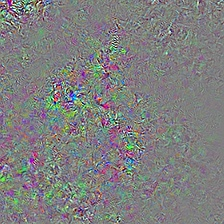
\includegraphics[width=.25\textwidth]{fig/gradient/fig/method/gradient.jpg}}; \&
		\node[box] (reg) {regularization \\ loss $L_R$}; \\
		\&\&\&\&\&\&\&
		\node[op] (plus) {$+$}; \&
		\node[txt] (loss) {total loss \\ $L = L_C + $\\ $\lambda L_R$}; \\
	};

	\draw[->]
		(in) edge (net)
		(net) edge node[above] {logits $y$} (class)
		(class) edge (back)
		(back) edge (grad)
		(guided-back) edge[sg] (guided)
		(grad) edge (reg)
		(reg) edge (plus)
		(plus) edge (loss)
		(class) edge[sg,out=90,in=180] (guided-back)
		(class) edge[loose,out=-50,in=180] (plus)
		(guided) edge[sg,out=0,in=90] node[pos=.2,font=\large,label=0:stop gradient] {//} (reg)
		(net) edge[dashed,out=60,in=150] (guided-back)
		(net) edge[dashed,out=30,in=150] (back)
		;
	\end{tikzpicture}
}